\section{DINOv2}
\label{sec:Chapter27}

DINOv2 je dalším z state-of-art přístupů představených v \cite{dinov2} roku 2023. Jedná se o model pod vlastním dohledem schopný dosáhnout řešit mnoho problémů počítačového vidění. Páteřní síť DINOv2 je síť s pomocí ViT pozornostních visuálních bloků (ang. Vision Transformer) \cite{vit}. Hlavní předtrénovaný model obsahuje přes 1 miliardu parametrů.

Model DINOv2 nachází uplatnění v řadě pokročilých úloh zpracování obrazu. Jeho využití je rozmanité a zahrnuje techniky jako segmentaci a klasifikaci, ale dokonce i odhad hloubky, párování typu dense matching nebo párování mezi sémanticky odpovídajícími klíčovými body (ang. sparse matching), vyobrazeno na obrázku \ref{fig:dinov2_sparse_matching}. Oba typy párování nachází relevantní části obrázku mezi sémanticky podobnými scénámi \cite{dinov2.metademolab.com}.

\begin{figure}[H]
\centering

\newcommand{\subfiguresize}{.15\textwidth}
\newcommand{\imagewidth}{1.0in}
\newcommand{\hspacesize}{.43in}

\newcommand{\insertimage}[1]{%
  \begin{minipage}{\imagewidth}
    \centering
    \includegraphics[width=\imagewidth]{#1}
  \end{minipage}
}

\subfloat[Ptáci / Letadla]{%
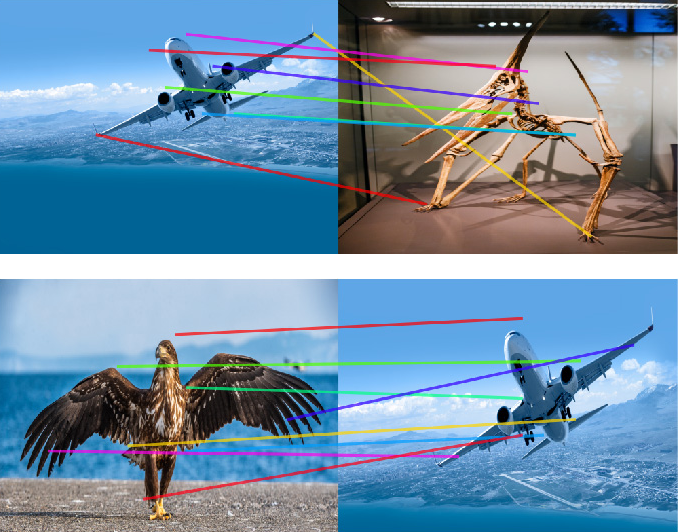
\includegraphics[width=0.4\textwidth,keepaspectratio]{Figures/dinov2_sparse_half_1.png}
  \label{fig:dinov2_birds_airplanes}%
}\hspace{\hspacesize}%
\subfloat[Vozidla]{%
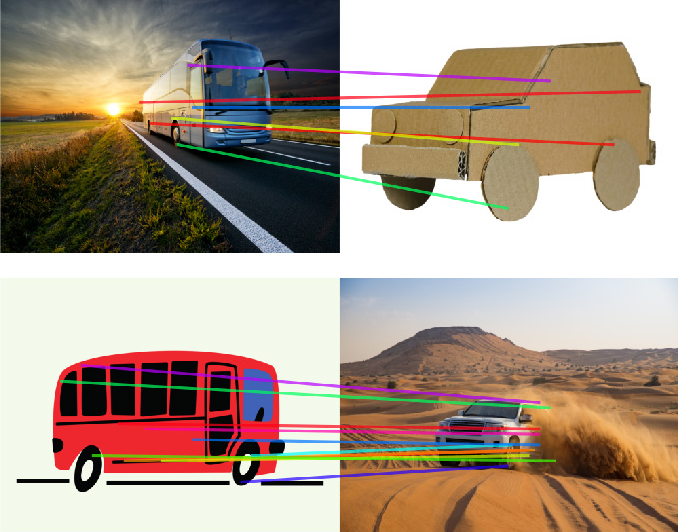
\includegraphics[width=0.4\textwidth,keepaspectratio]{Figures/dinov2_sparse_half_2.png}
  \label{fig:dinov2_vehicles}%
}

\caption[Využití DINOv2 pro párování typu sparse matching]
{Využití DINOv2 pro párování typu sparse matching mezi sémanticky podobnými scénami. Převzato z \cite{dinov2} a přeloženo.}
\label{fig:dinov2_sparse_matching}
\end{figure}

\endinput